% Figures for the project book.
% Keep the book_figures folder next to your main .tex file and add \usepackage{graphicx} to the preamble.
% \listoffigures in the front matter builds the LIST OF FIGURES from these captions automatically.
% Place each figure in the chapter where it is discussed and cite it with \ref{label}.

\begin{figure}[htbp]
  \centering
  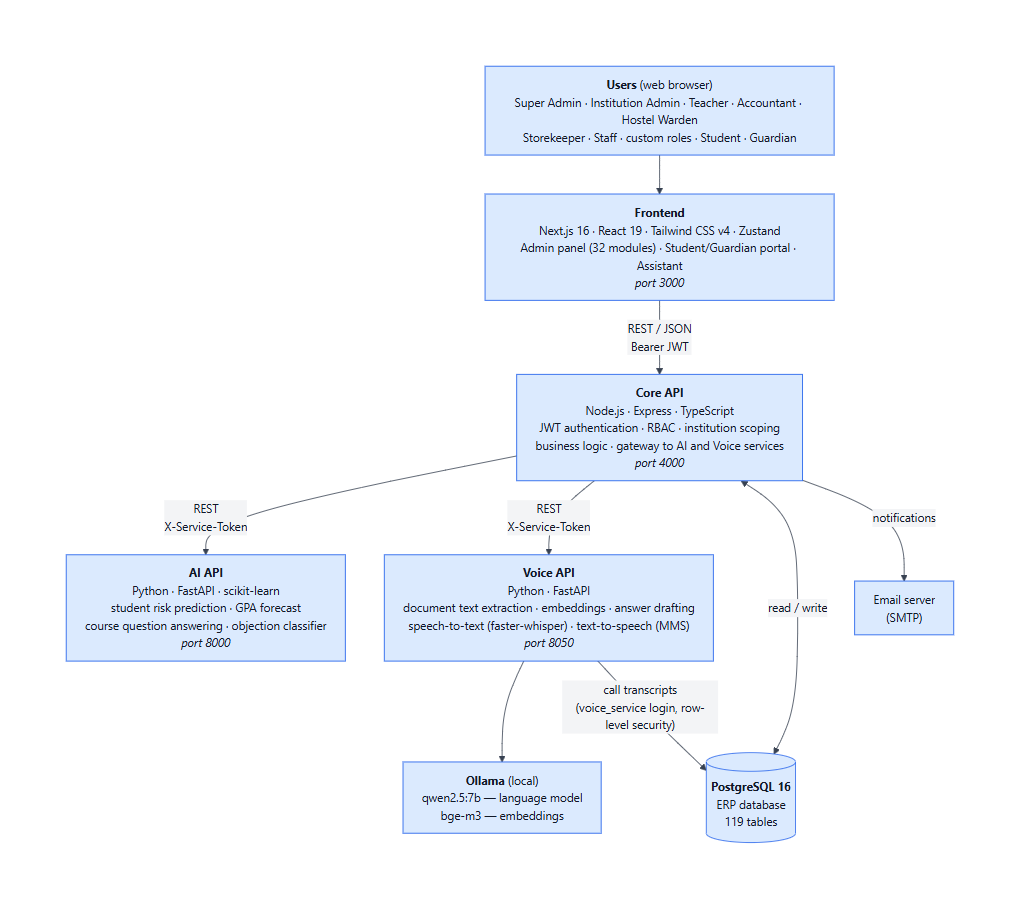
\includegraphics[width=\textwidth,height=0.85\textheight,keepaspectratio]{book_figures/fig01_system_architecture.png}
  \caption{Overall system architecture of the platform}
  \label{fig:architecture}
\end{figure}

\begin{figure}[htbp]
  \centering
  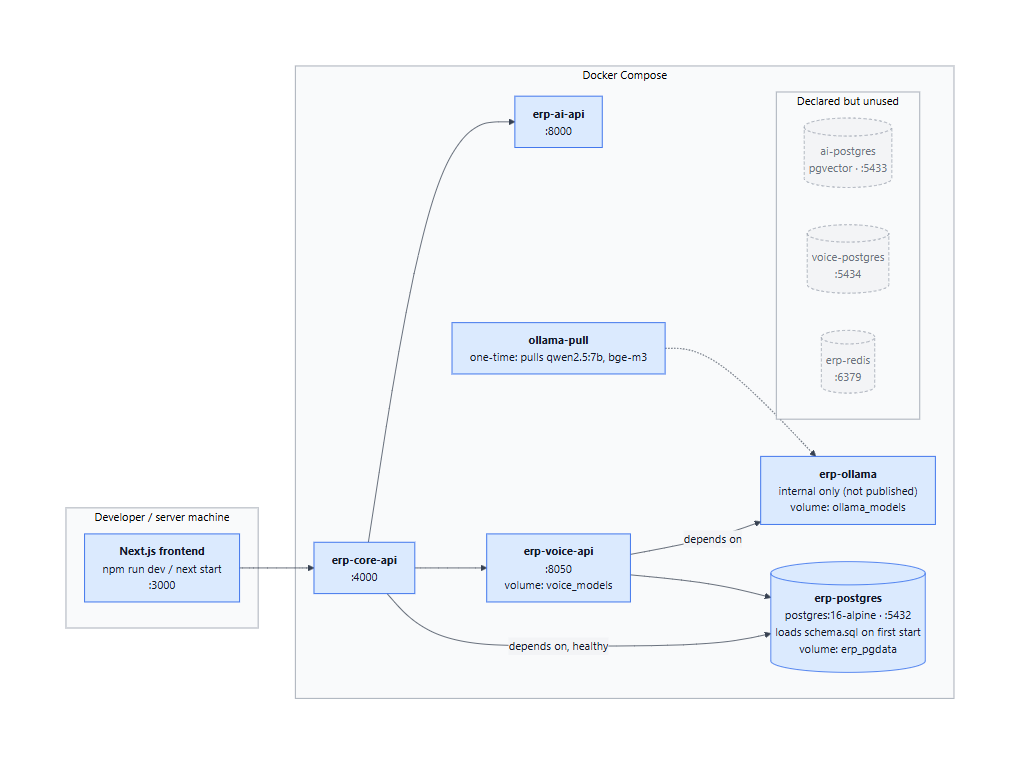
\includegraphics[width=\textwidth,height=0.85\textheight,keepaspectratio]{book_figures/fig02_deployment.png}
  \caption{Container deployment with Docker Compose}
  \label{fig:deployment}
\end{figure}

\begin{figure}[htbp]
  \centering
  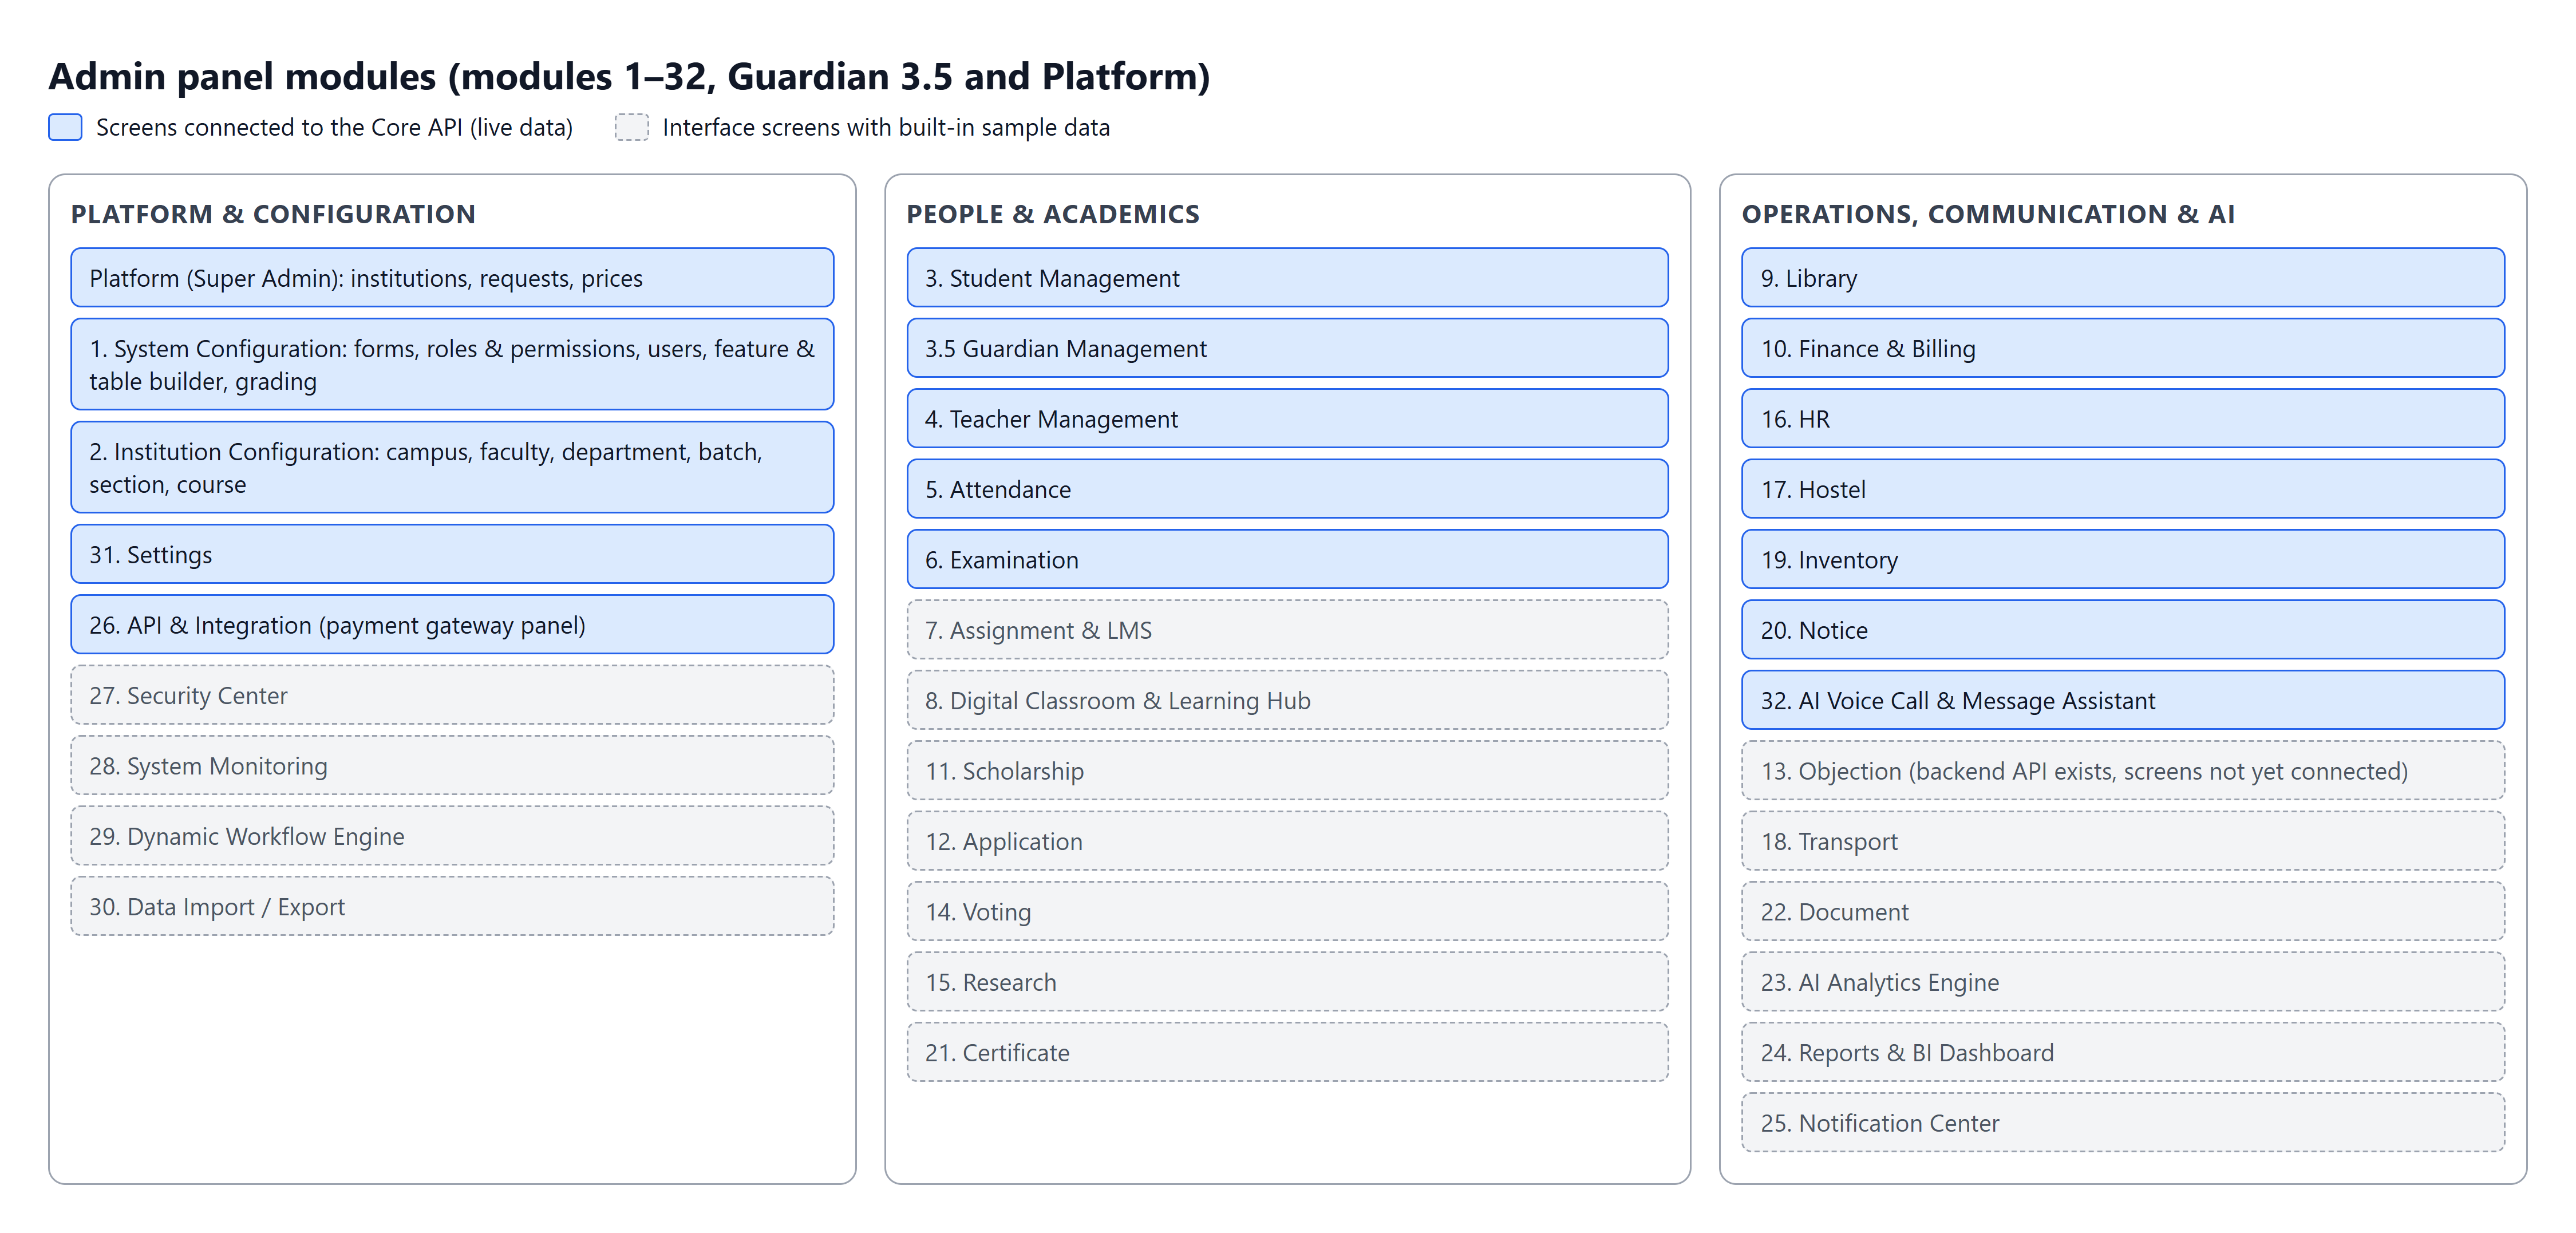
\includegraphics[width=\textwidth,height=0.85\textheight,keepaspectratio]{book_figures/fig03_module_map.png}
  \caption{Admin panel module map and integration status}
  \label{fig:modules}
\end{figure}

\begin{figure}[htbp]
  \centering
  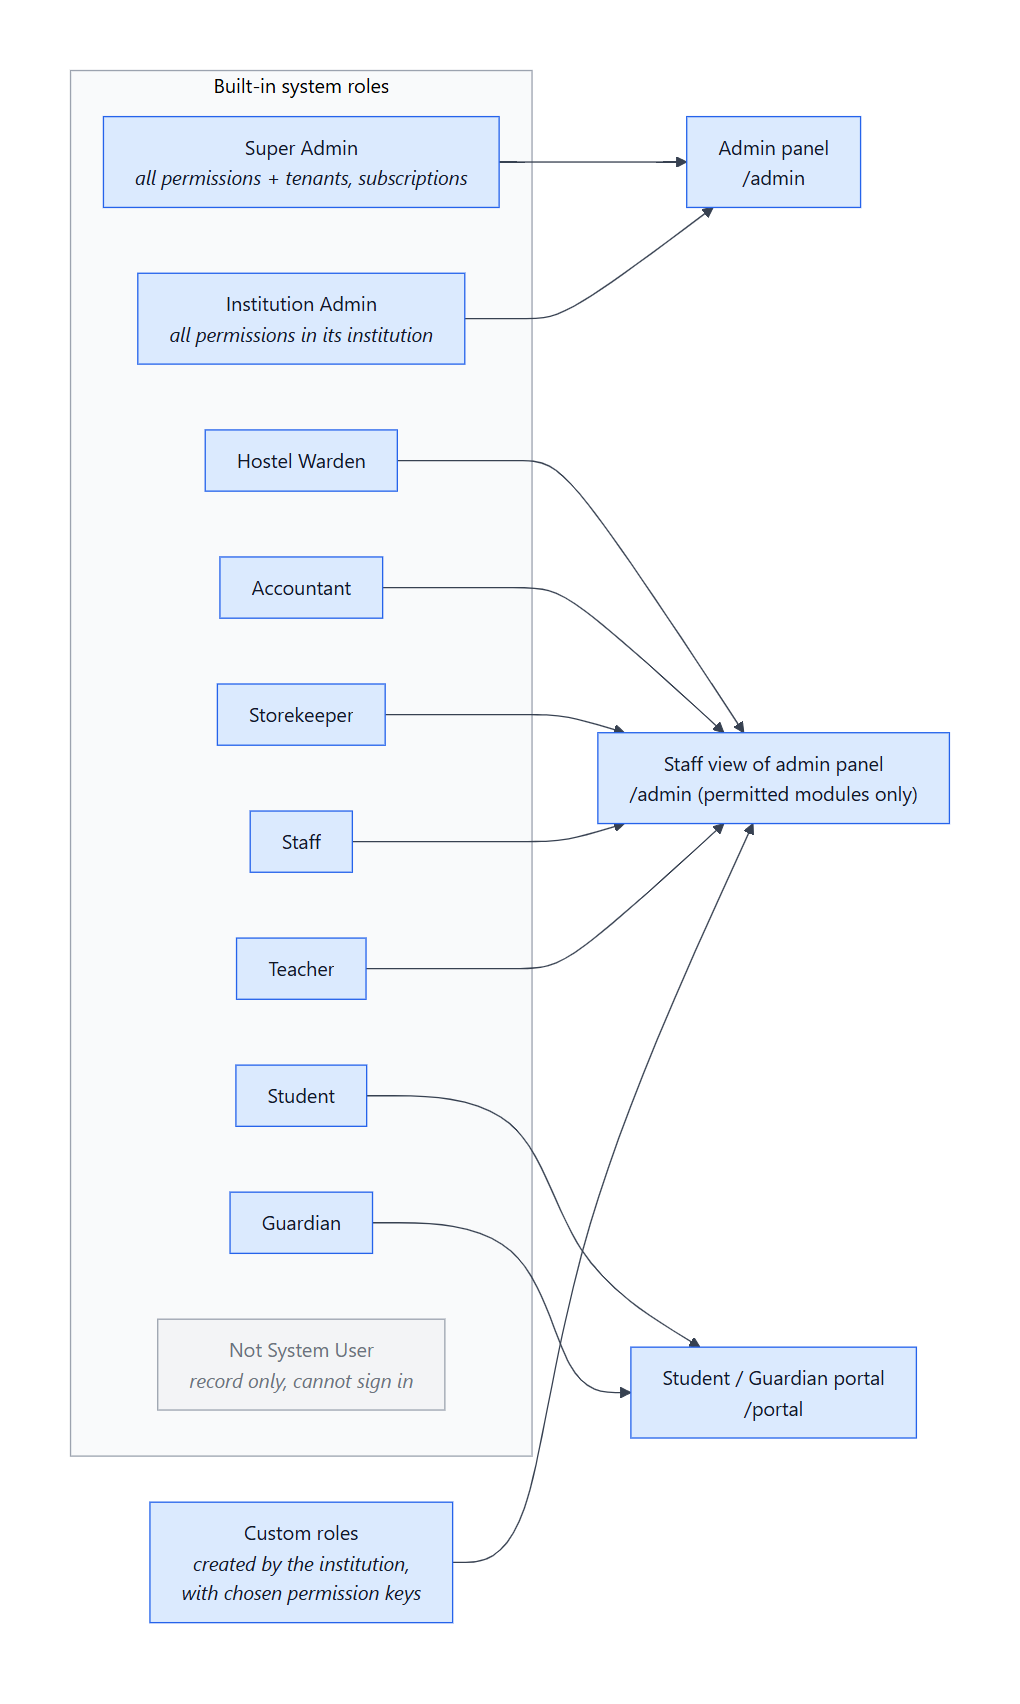
\includegraphics[width=0.75\textwidth,height=0.85\textheight,keepaspectratio]{book_figures/fig04_roles_portals.png}
  \caption{Built-in user roles and the portals they use}
  \label{fig:roles}
\end{figure}

\begin{figure}[htbp]
  \centering
  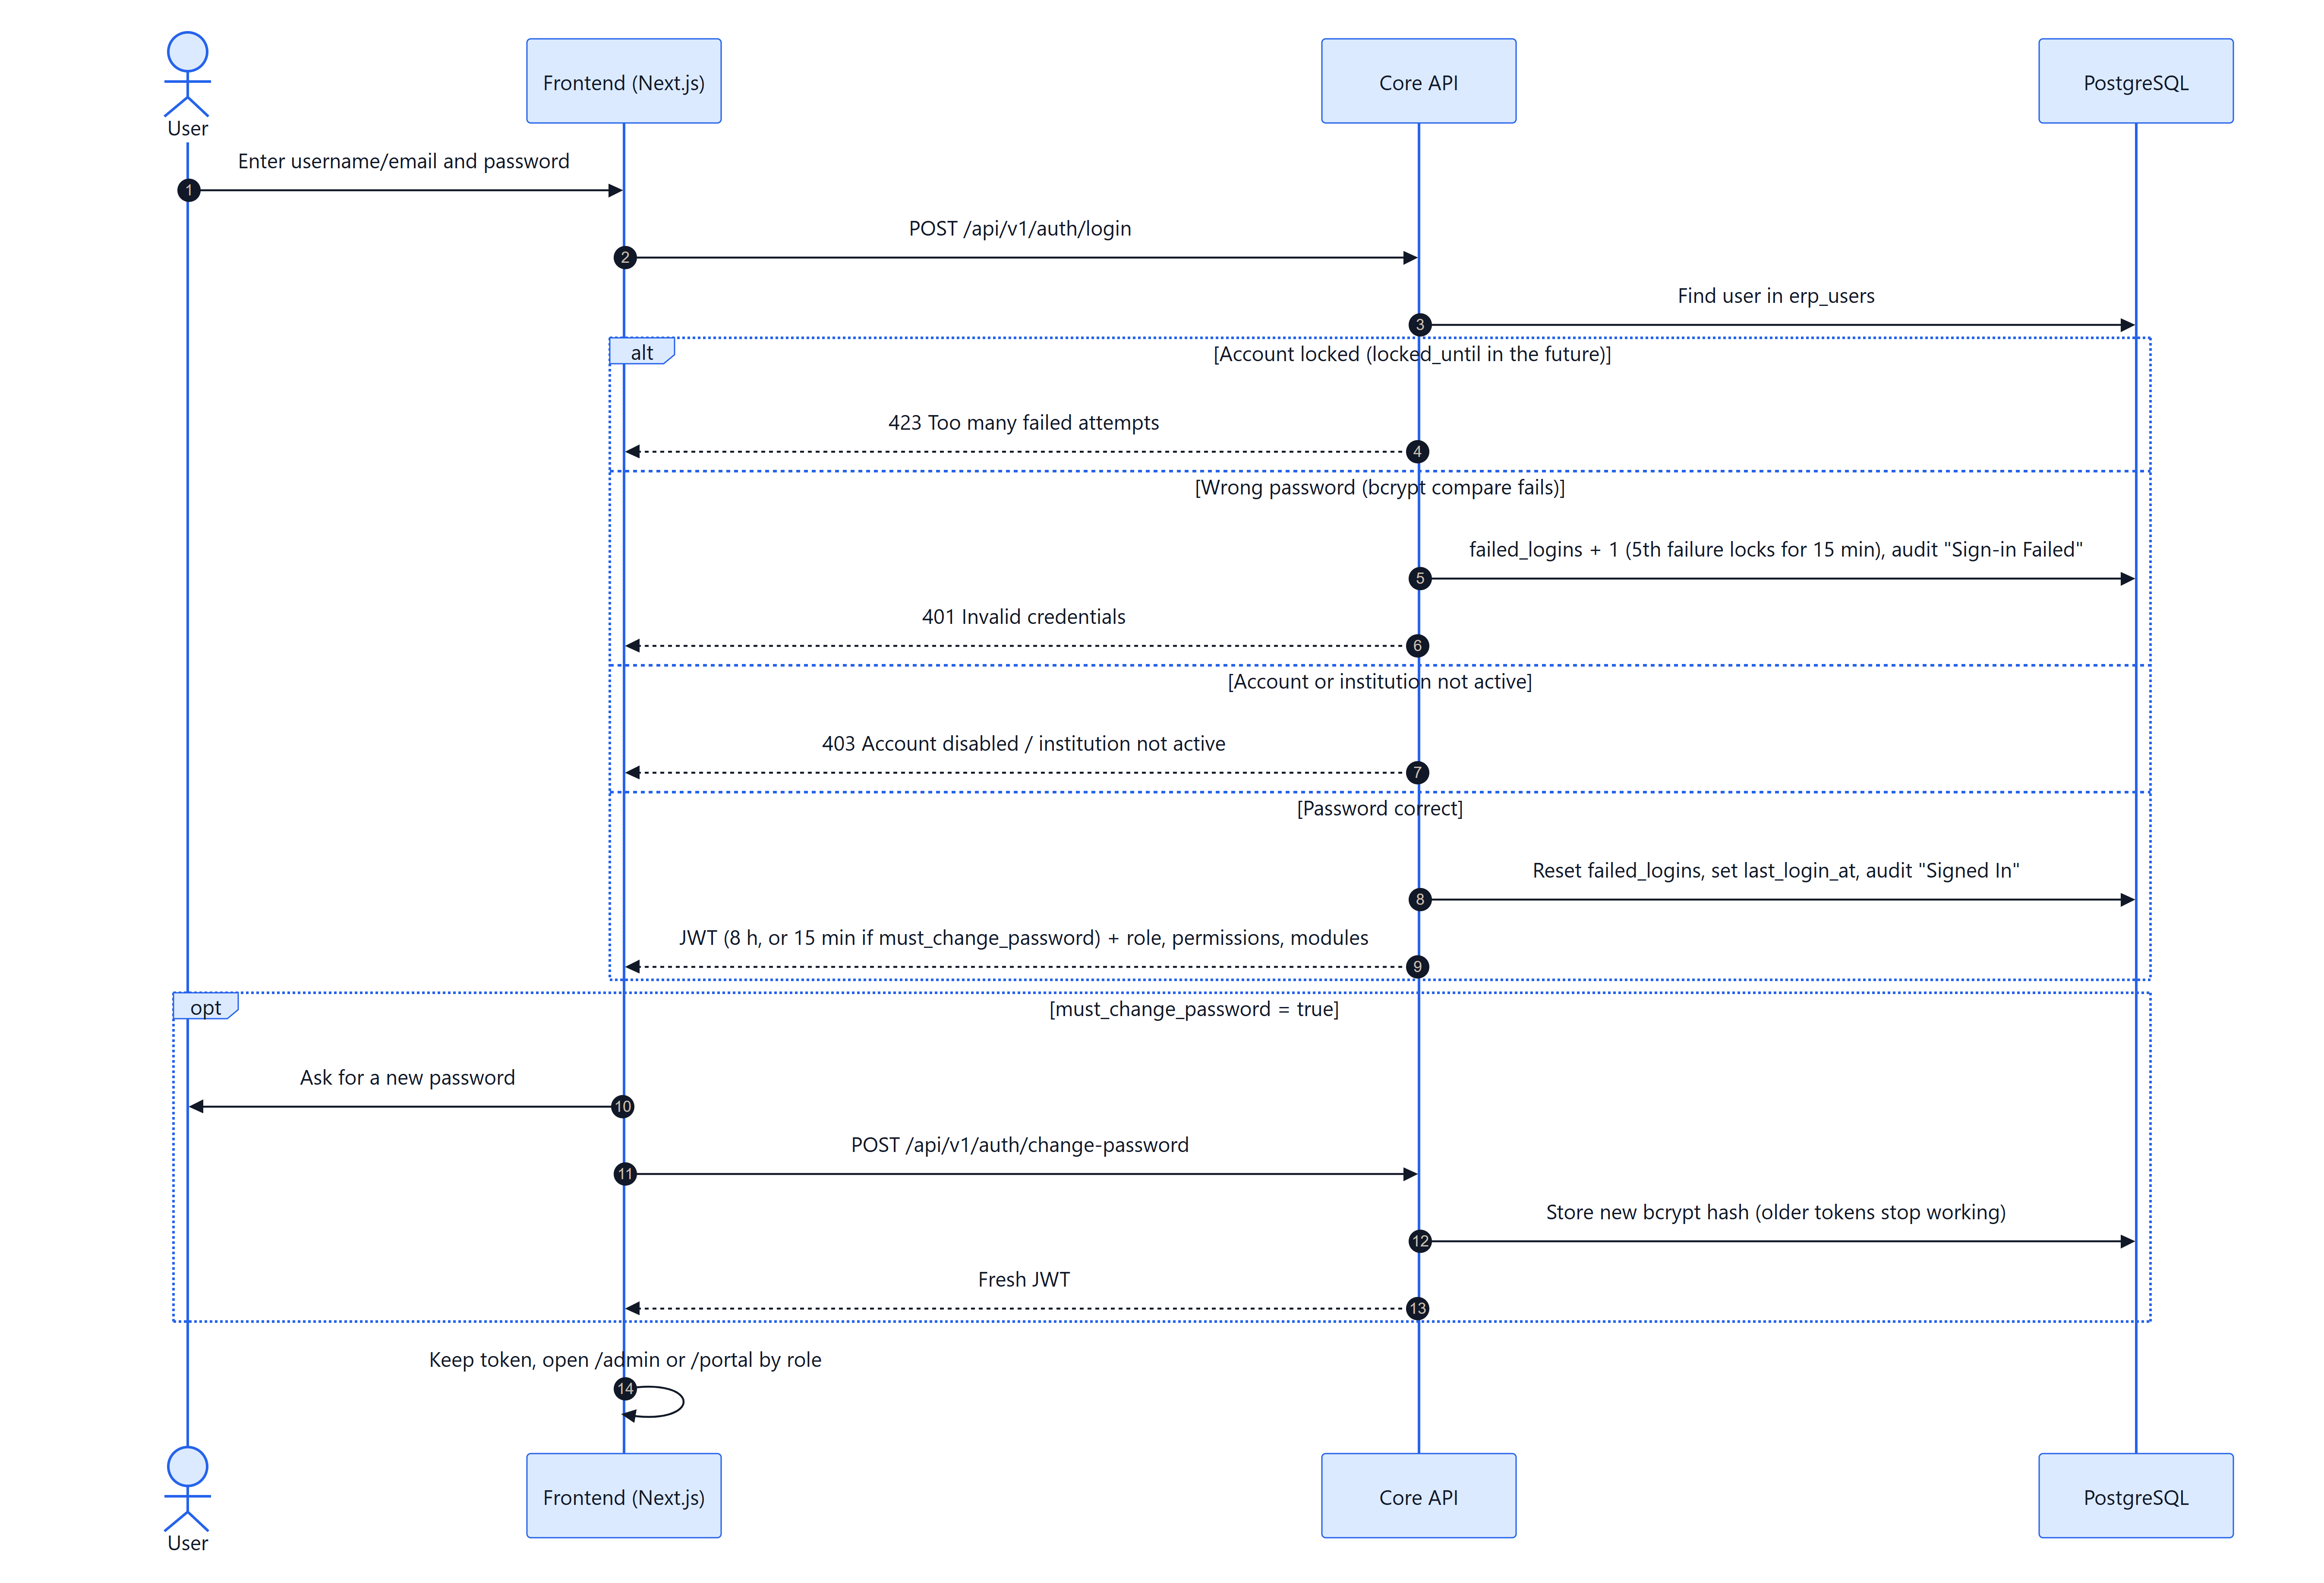
\includegraphics[width=\textwidth,height=0.85\textheight,keepaspectratio]{book_figures/fig05_login_sequence.png}
  \caption{Sign-in and temporary password change sequence}
  \label{fig:login}
\end{figure}

\begin{figure}[htbp]
  \centering
  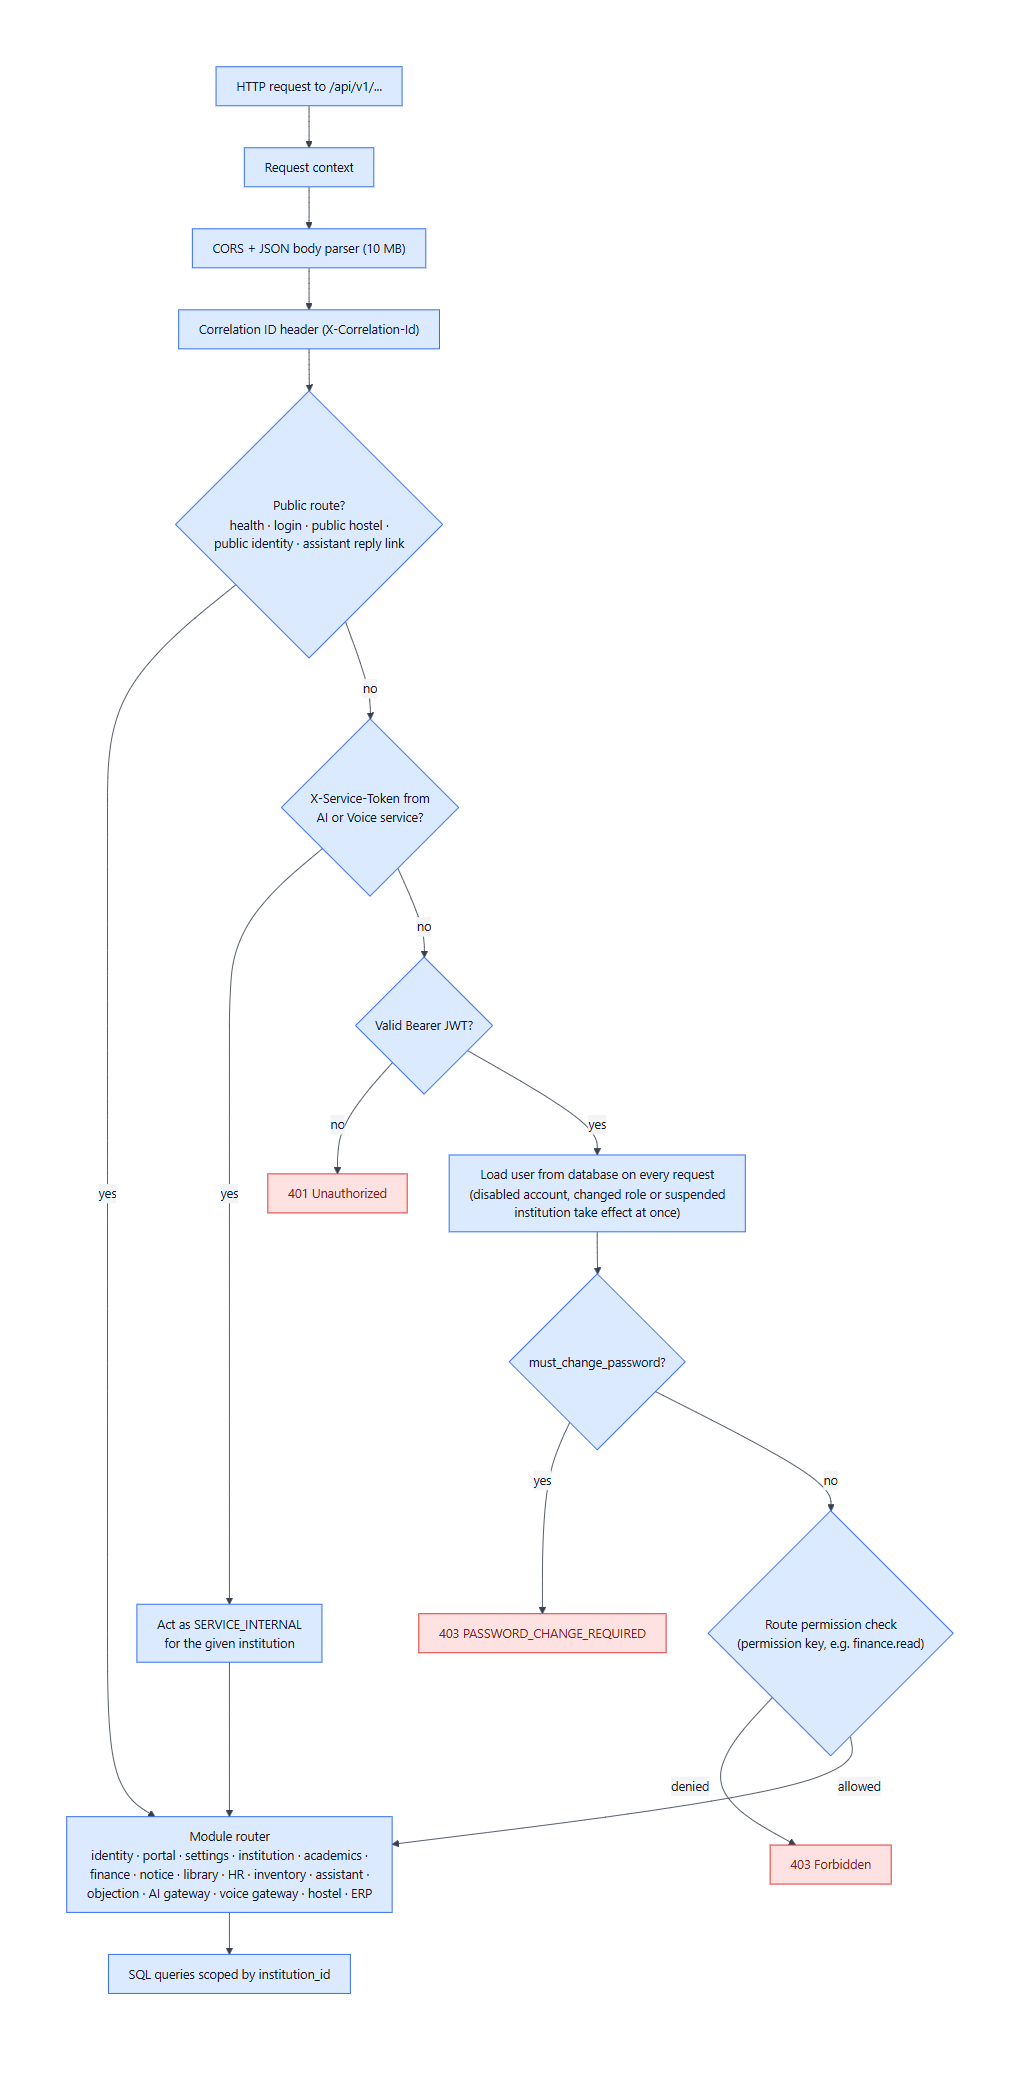
\includegraphics[width=0.7\textwidth,height=0.85\textheight,keepaspectratio]{book_figures/fig06_request_pipeline.png}
  \caption{Core API request authentication and authorisation pipeline}
  \label{fig:pipeline}
\end{figure}

\begin{figure}[htbp]
  \centering
  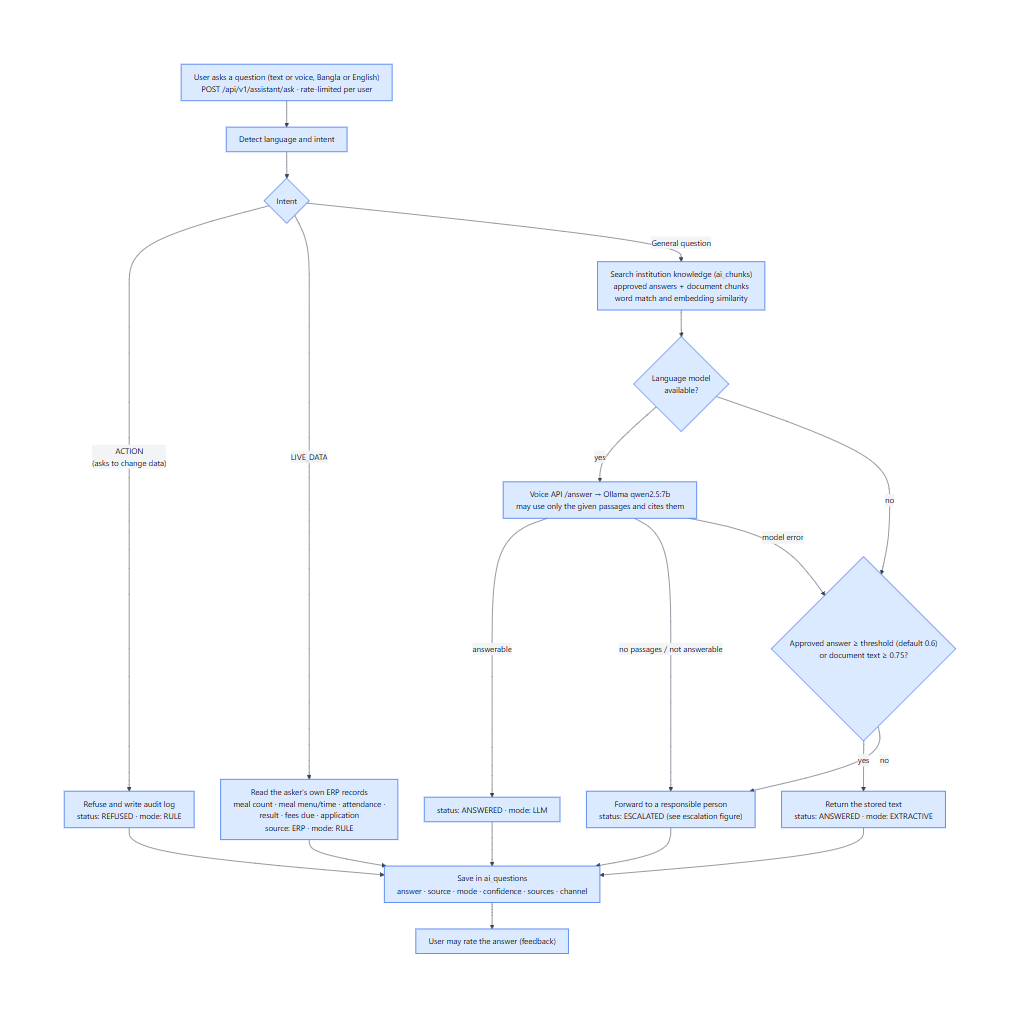
\includegraphics[width=\textwidth,height=0.85\textheight,keepaspectratio]{book_figures/fig07_assistant_answer_flow.png}
  \caption{Message assistant question answering flow}
  \label{fig:assistant}
\end{figure}

\begin{figure}[htbp]
  \centering
  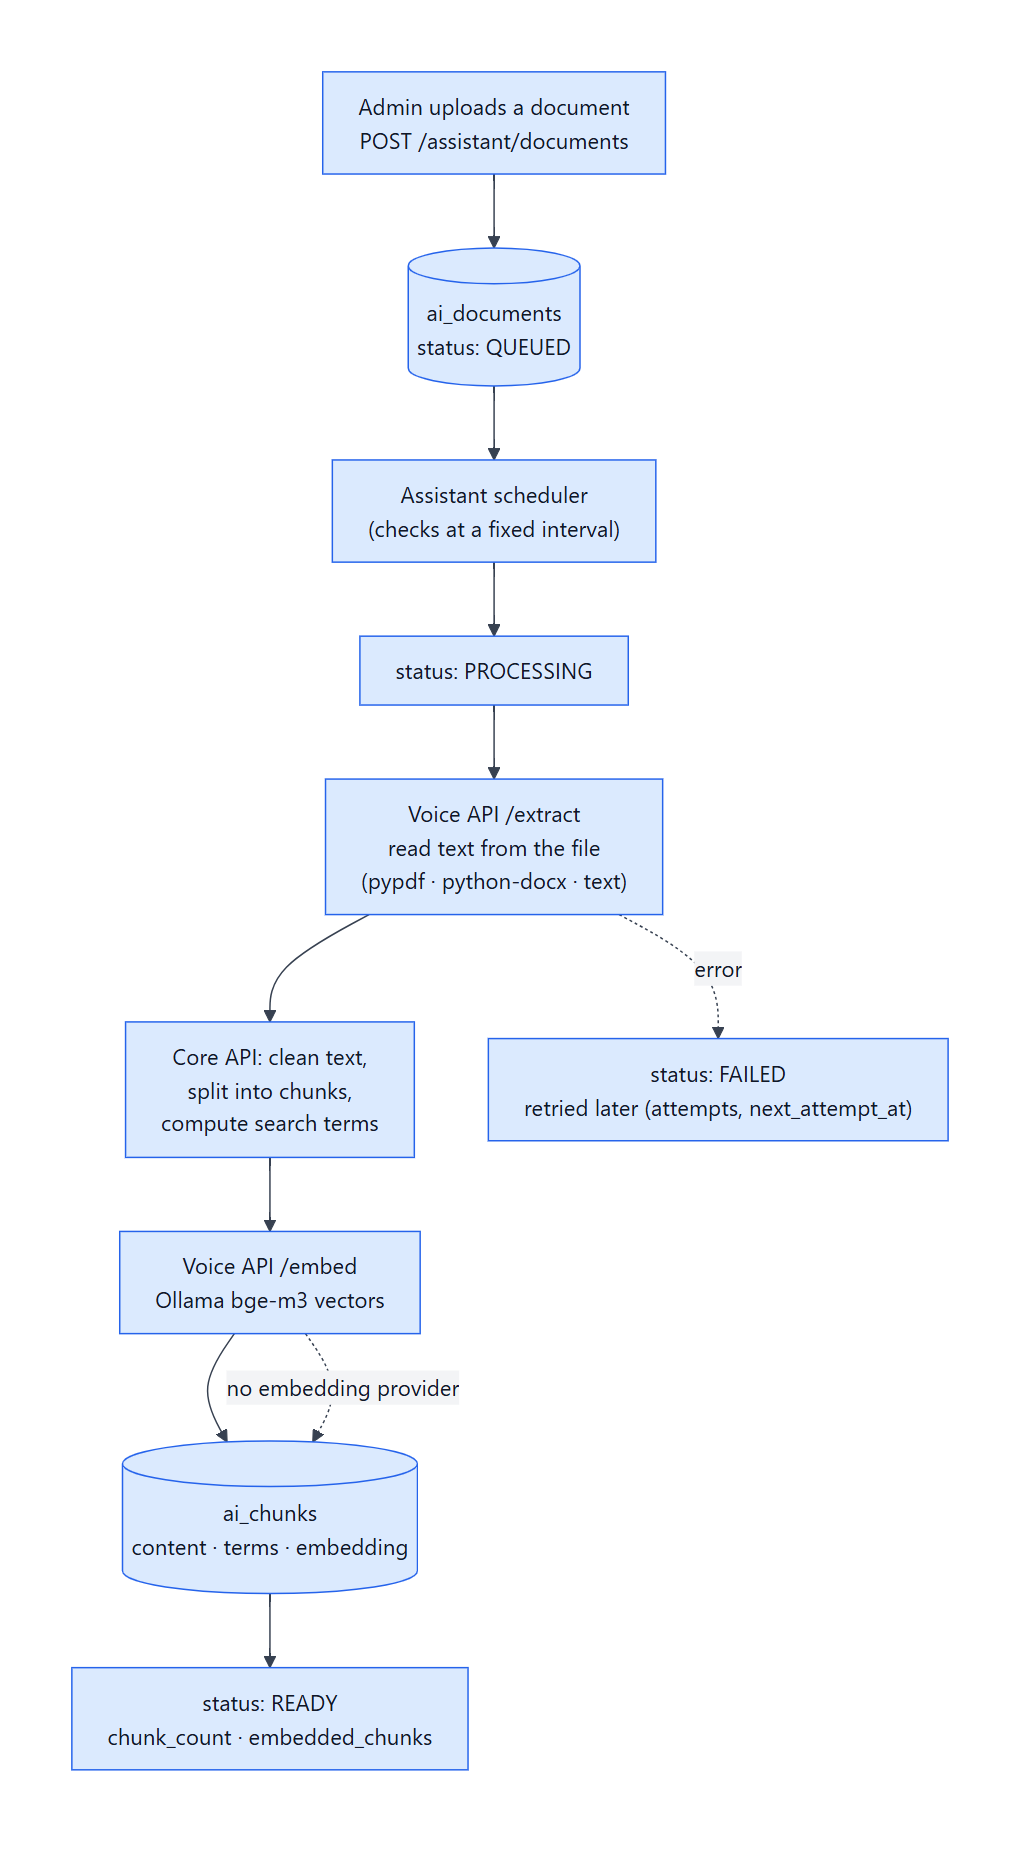
\includegraphics[width=0.6\textwidth,height=0.85\textheight,keepaspectratio]{book_figures/fig08_document_ingestion.png}
  \caption{Knowledge document ingestion pipeline}
  \label{fig:ingestion}
\end{figure}

\begin{figure}[htbp]
  \centering
  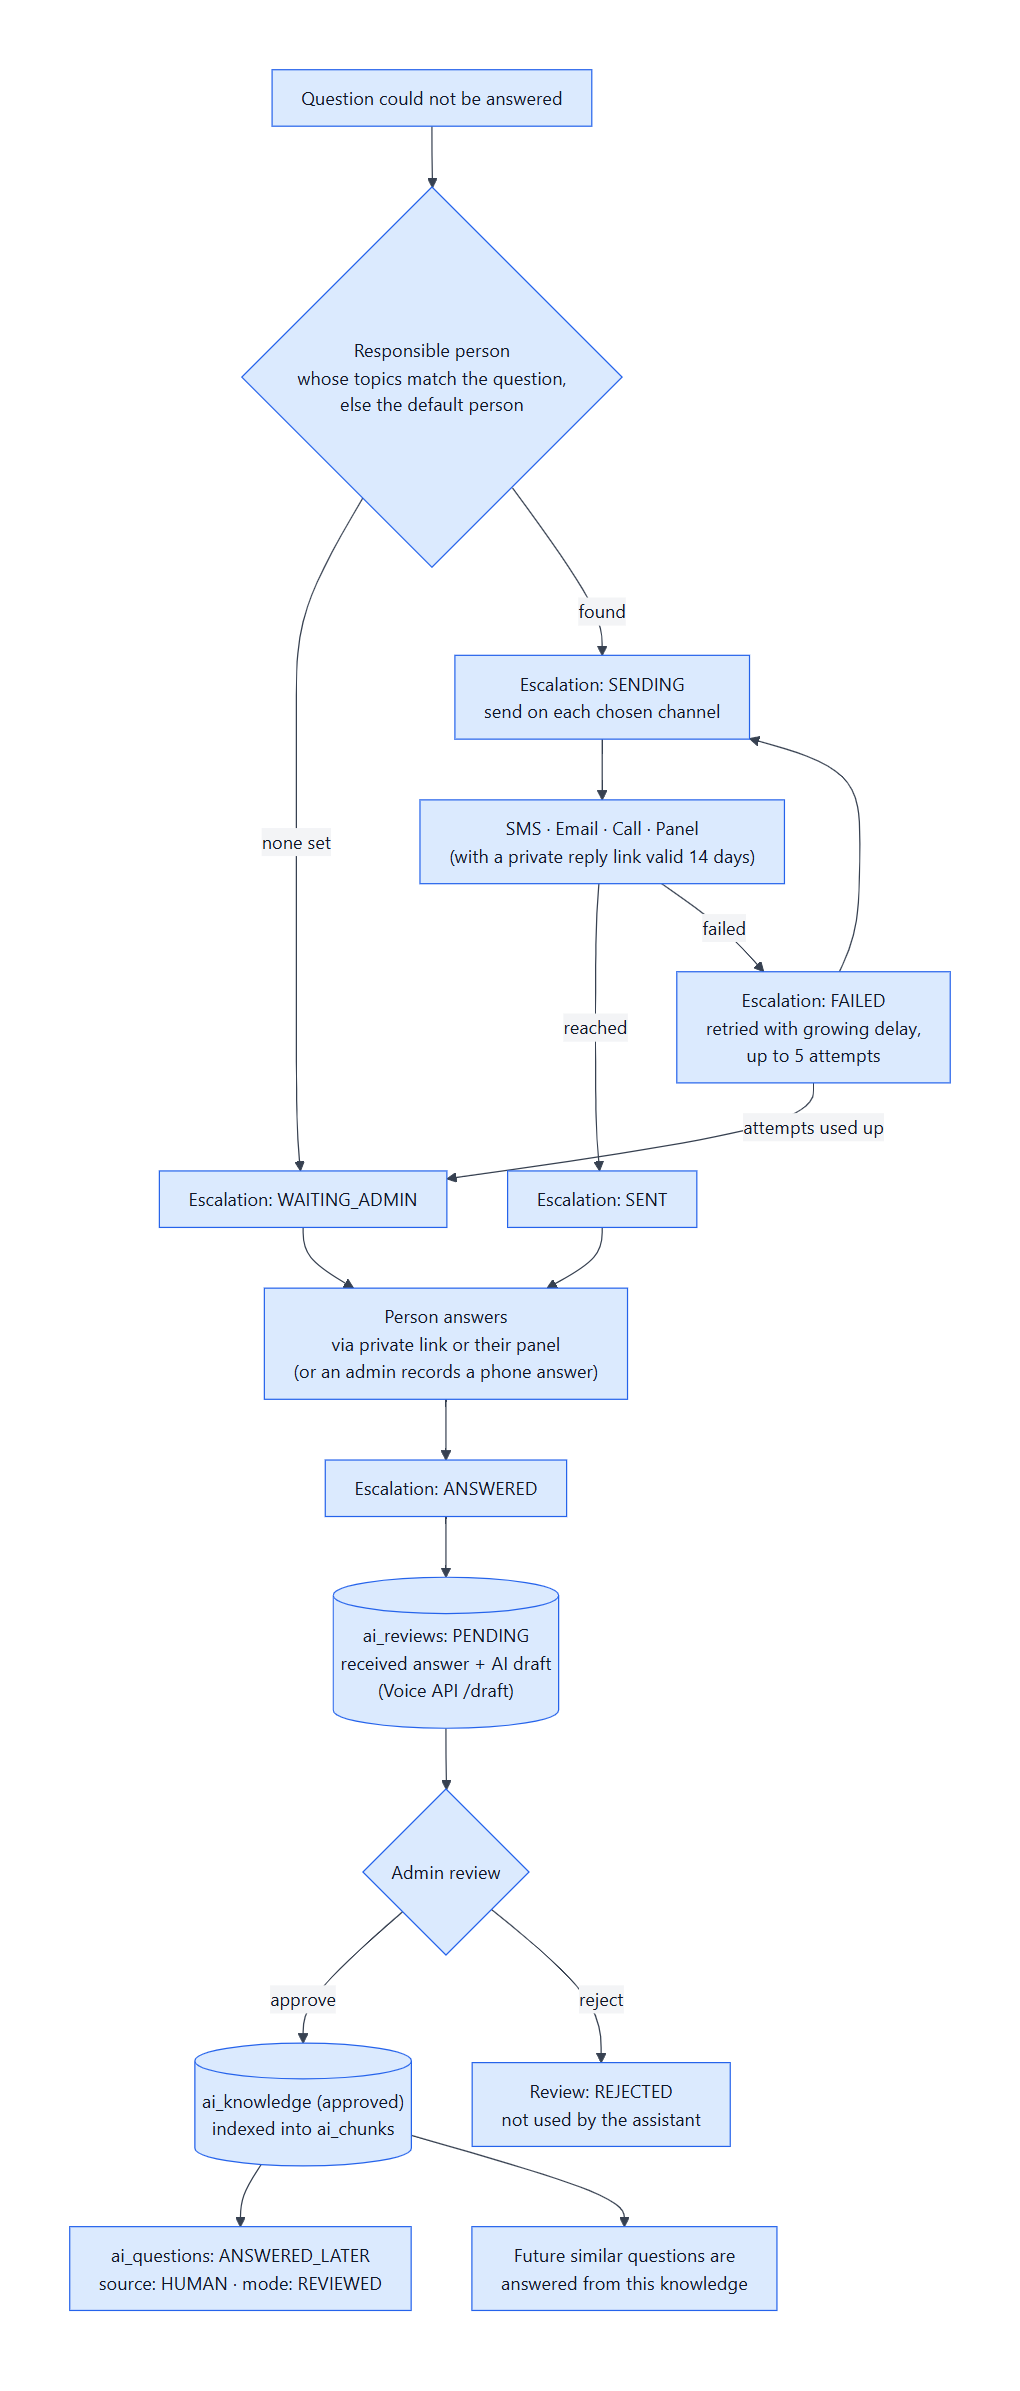
\includegraphics[width=0.75\textwidth,height=0.85\textheight,keepaspectratio]{book_figures/fig09_escalation_review.png}
  \caption{Escalation of unanswered questions and admin review}
  \label{fig:escalation}
\end{figure}

\begin{figure}[htbp]
  \centering
  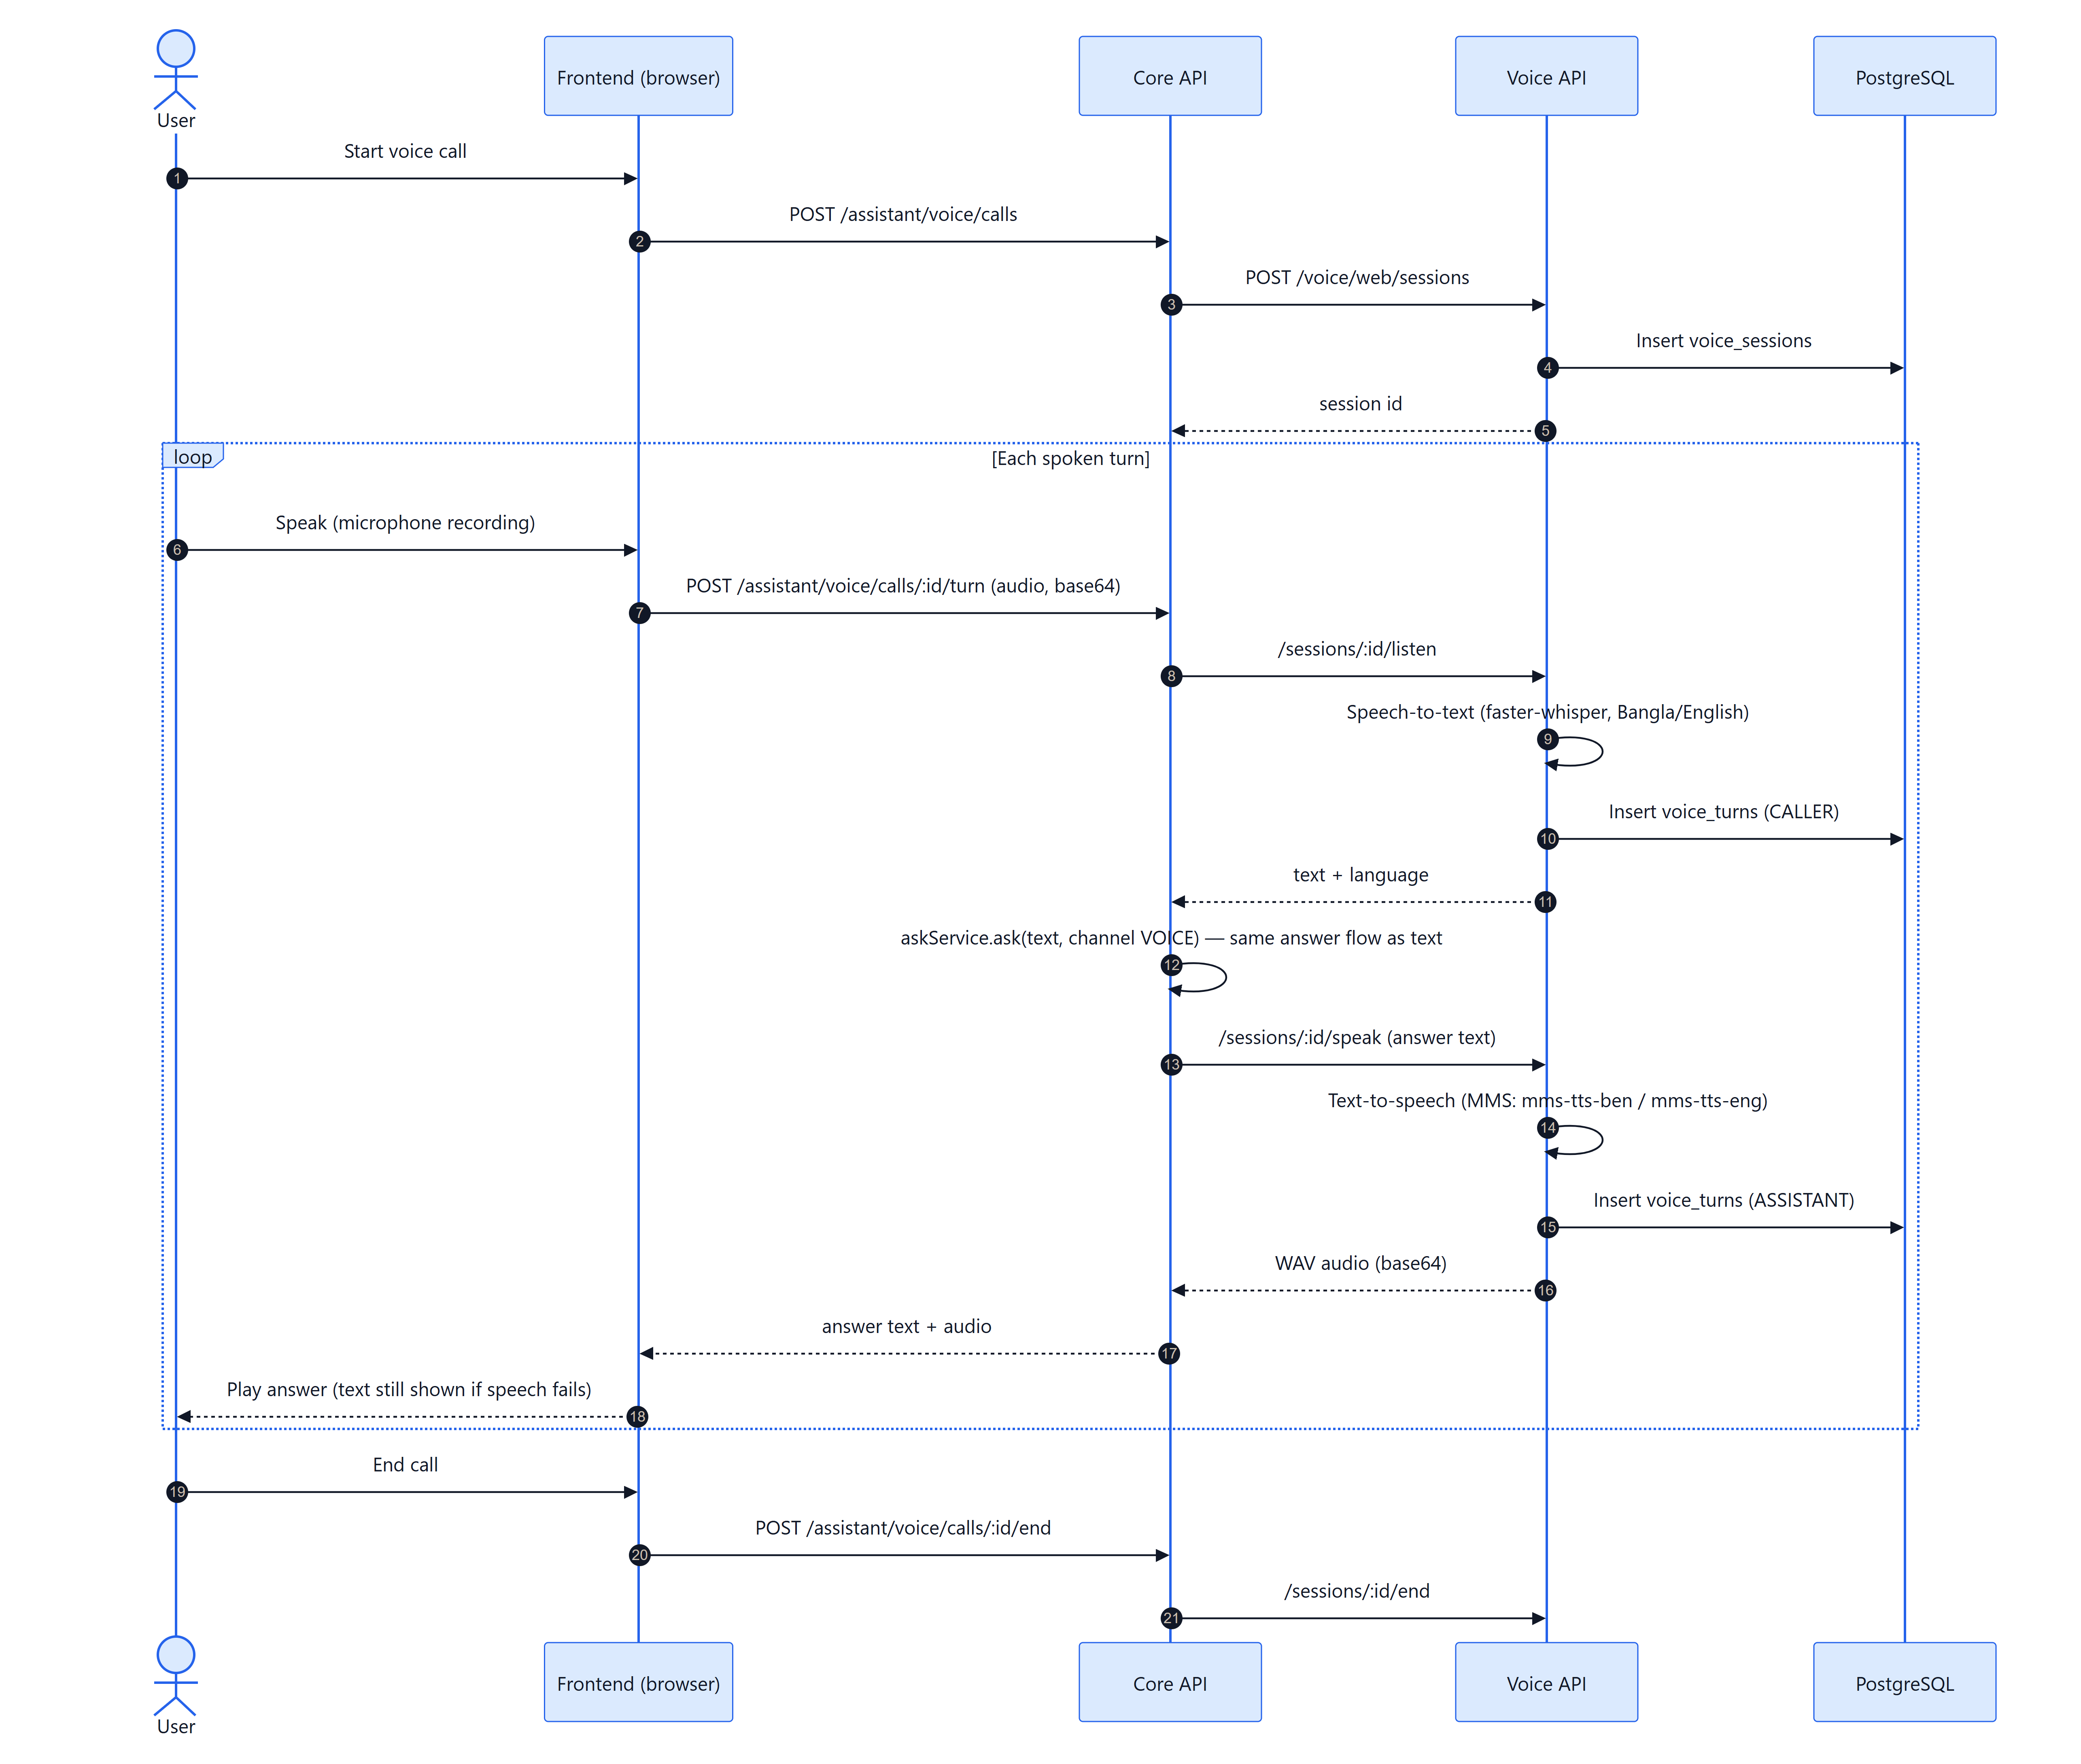
\includegraphics[width=\textwidth,height=0.85\textheight,keepaspectratio]{book_figures/fig10_voice_call_sequence.png}
  \caption{Voice call sequence between the browser, Core API and Voice API}
  \label{fig:voice}
\end{figure}

\begin{figure}[htbp]
  \centering
  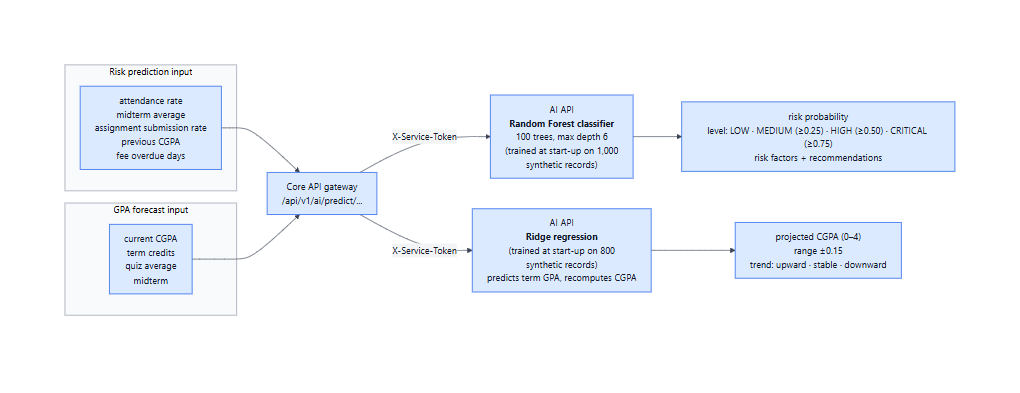
\includegraphics[width=\textwidth,height=0.85\textheight,keepaspectratio]{book_figures/fig11_ai_prediction.png}
  \caption{Student risk prediction and GPA forecast models}
  \label{fig:prediction}
\end{figure}

\begin{figure}[htbp]
  \centering
  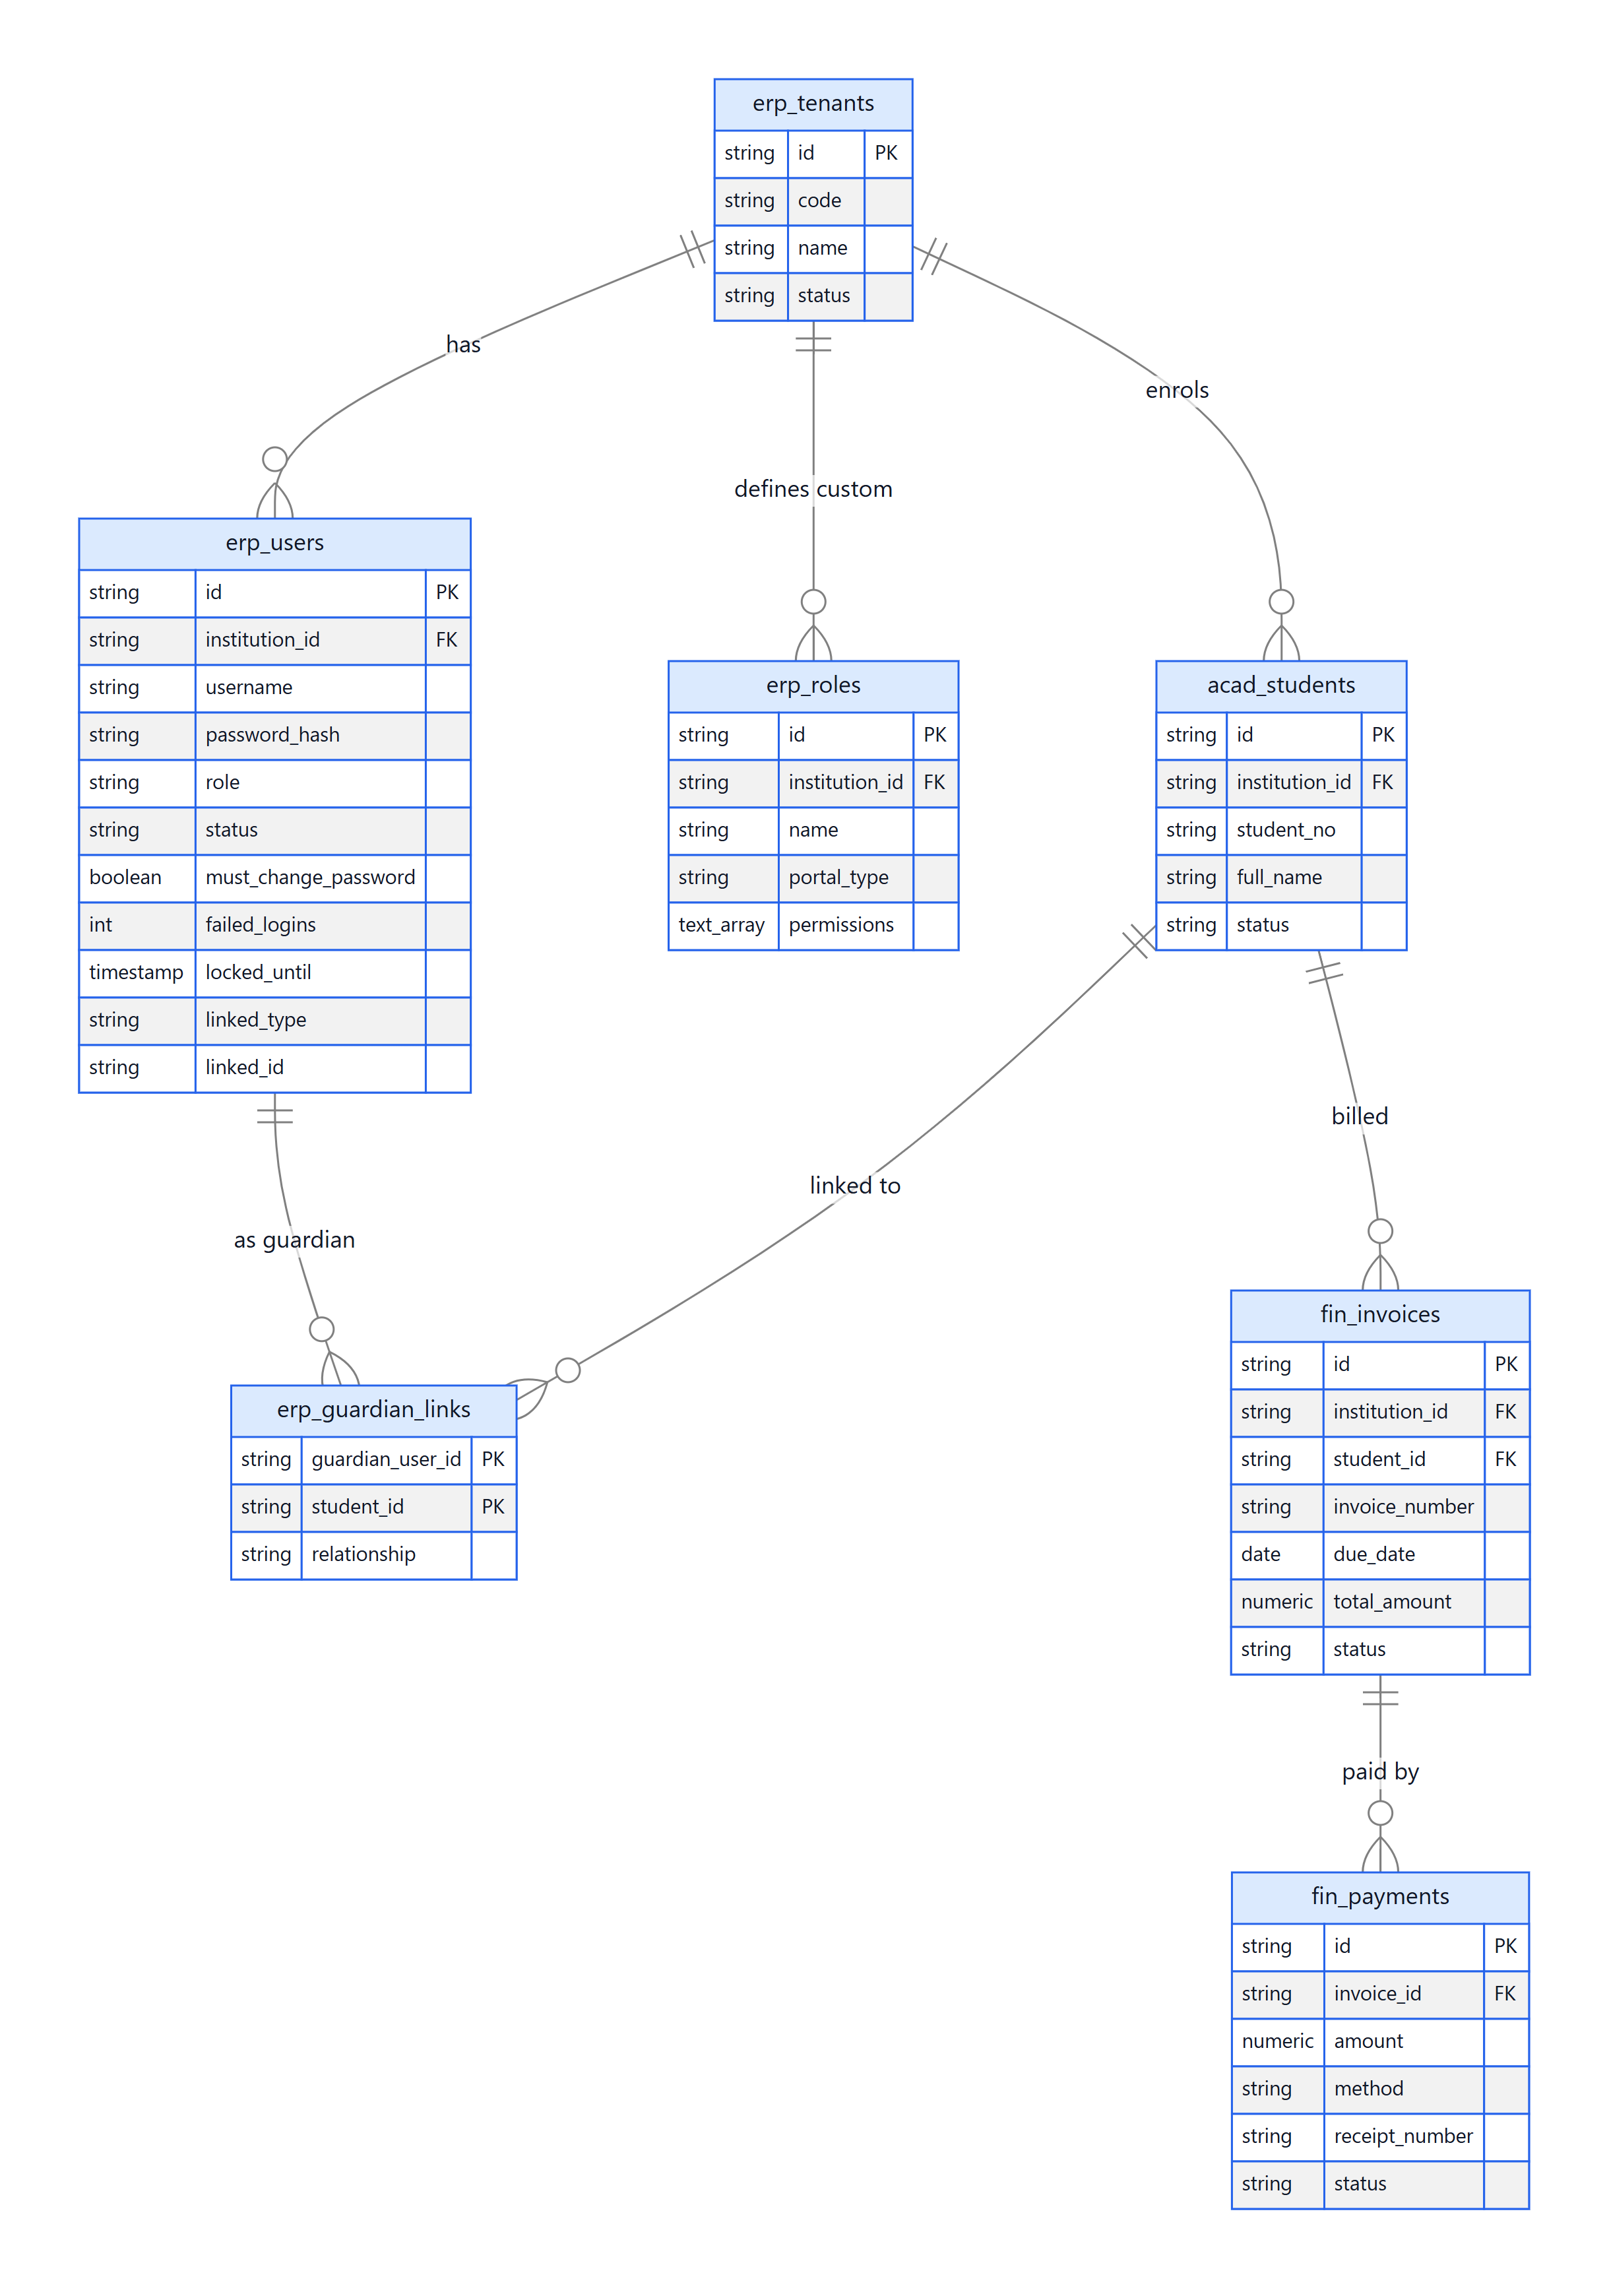
\includegraphics[width=0.8\textwidth,height=0.85\textheight,keepaspectratio]{book_figures/fig12_erd_identity_finance.png}
  \caption{Entity--relationship diagram: identity, guardians and finance}
  \label{fig:erd-identity}
\end{figure}

\begin{figure}[htbp]
  \centering
  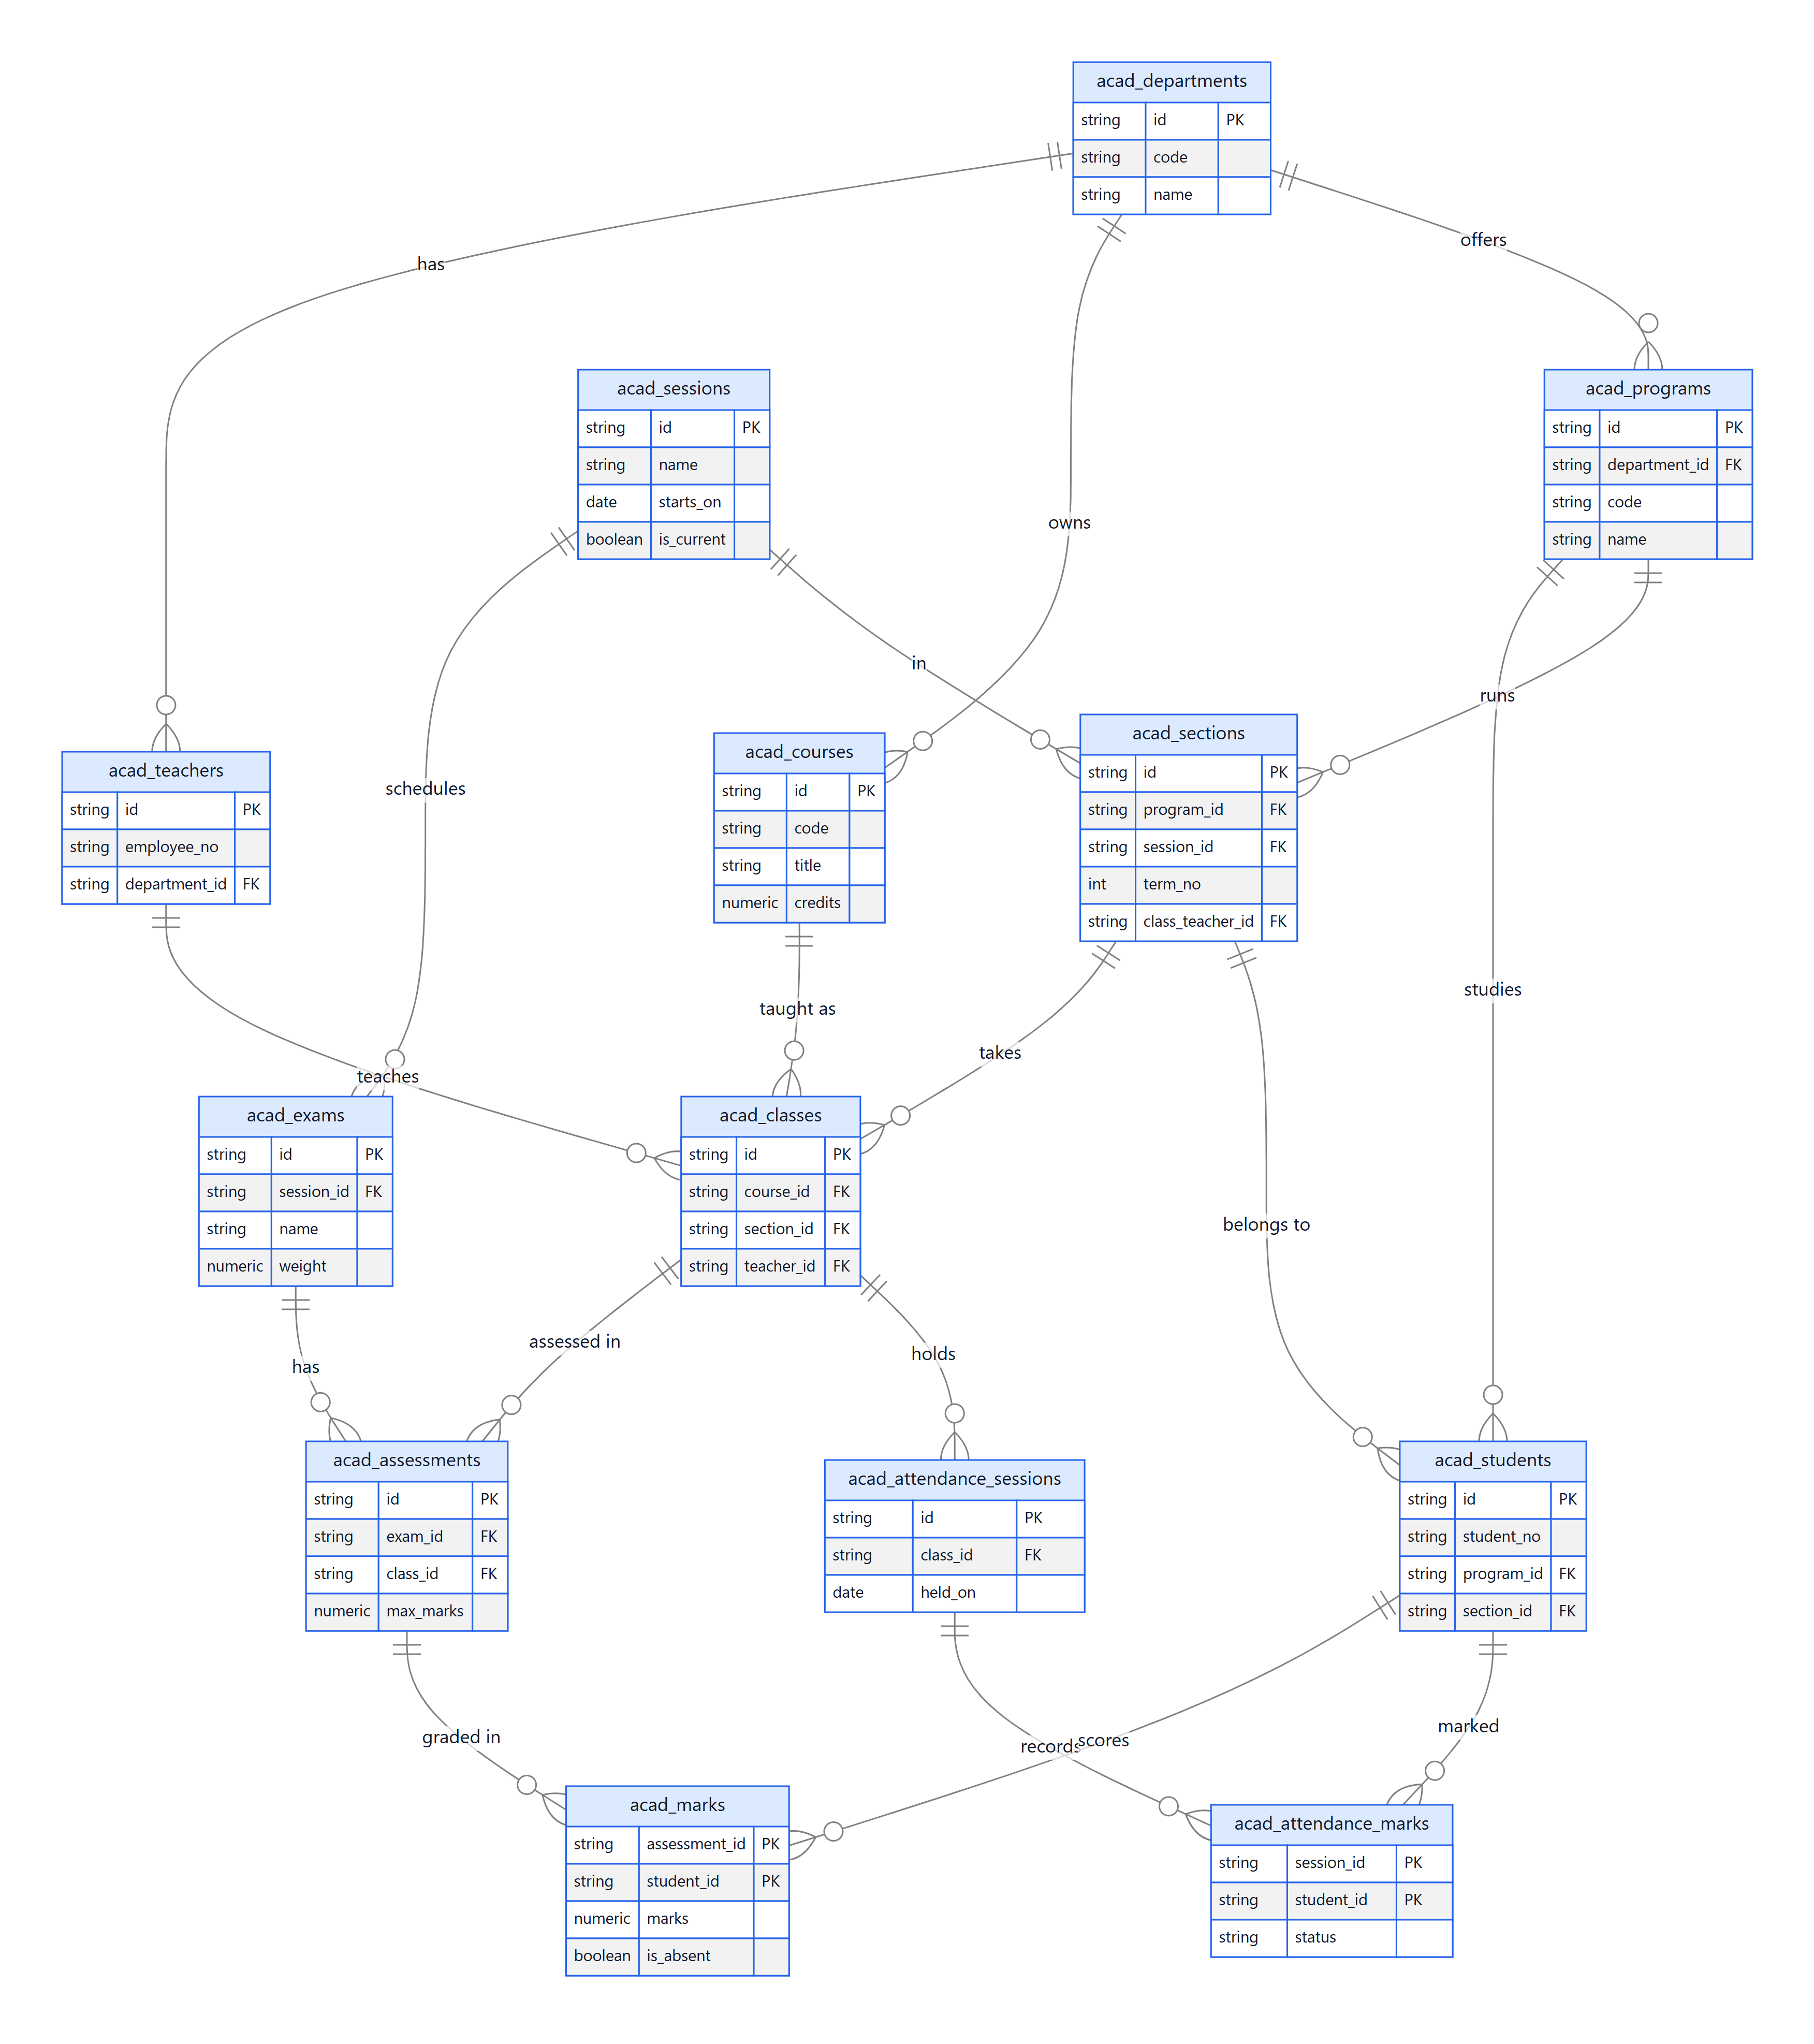
\includegraphics[width=\textwidth,height=0.85\textheight,keepaspectratio]{book_figures/fig13_erd_academics.png}
  \caption{Entity--relationship diagram: academic structure, attendance and marks}
  \label{fig:erd-academics}
\end{figure}

\begin{figure}[htbp]
  \centering
  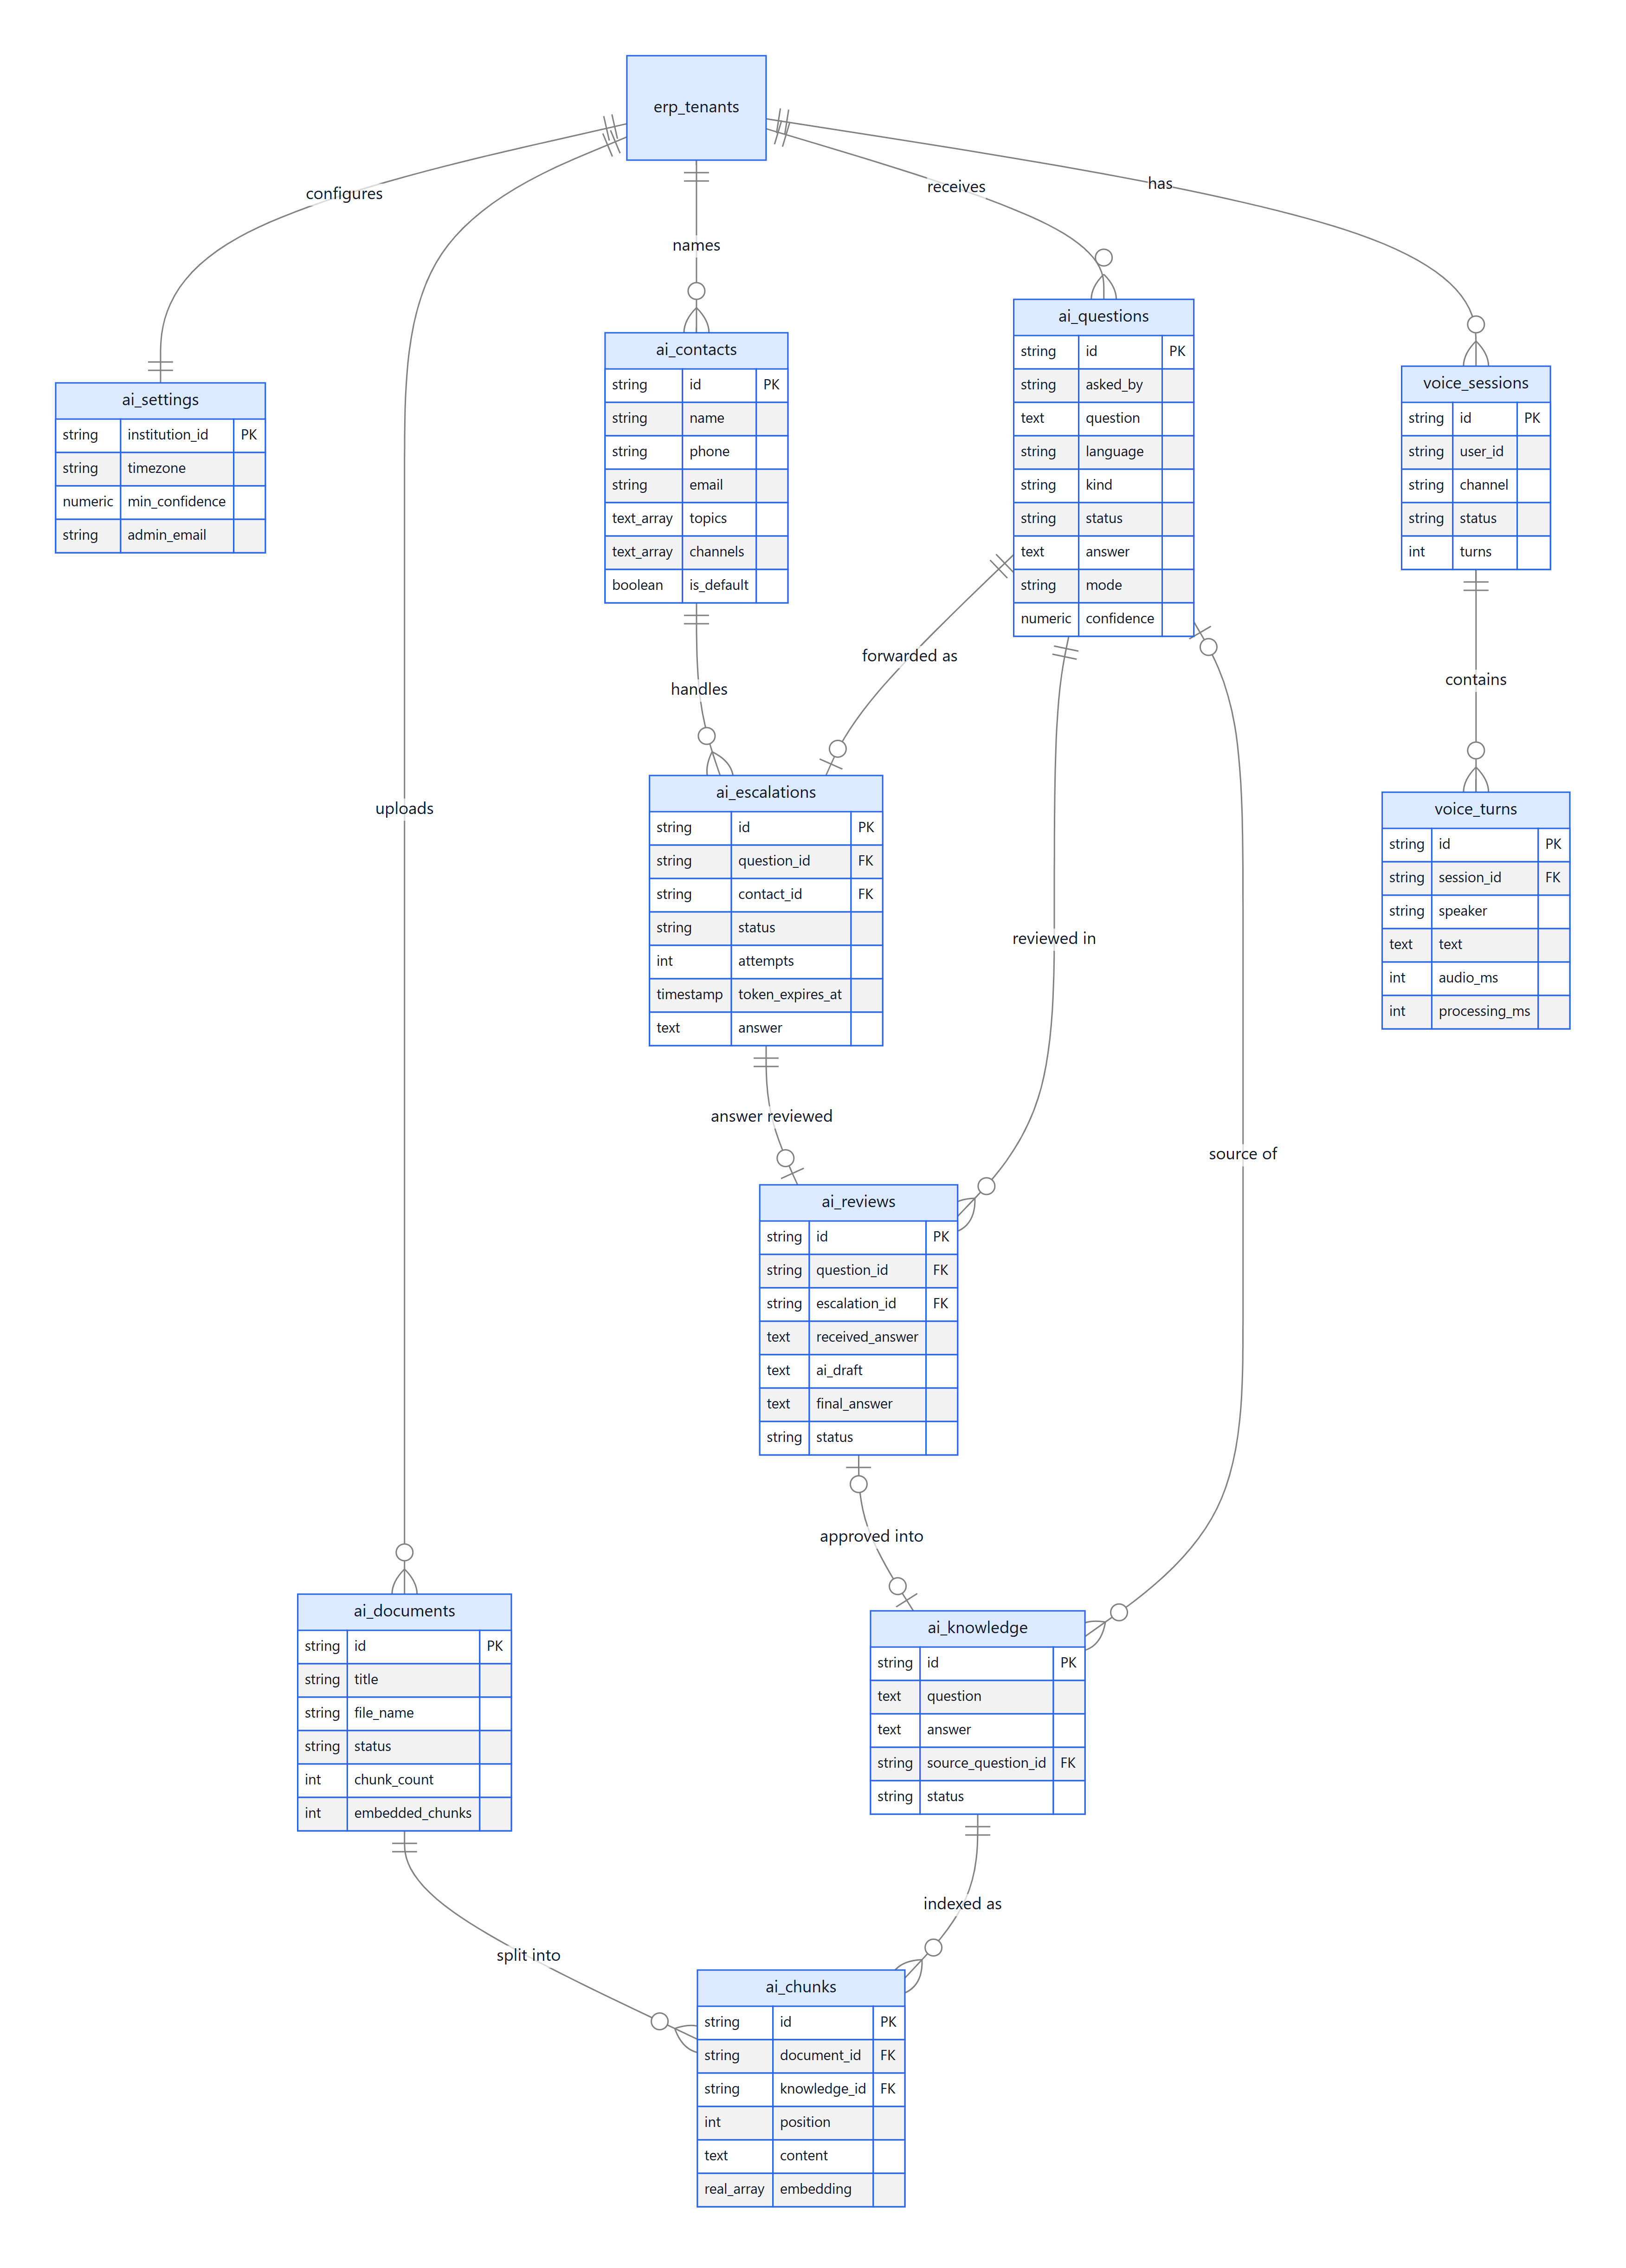
\includegraphics[width=0.85\textwidth,height=0.85\textheight,keepaspectratio]{book_figures/fig14_erd_assistant.png}
  \caption{Entity--relationship diagram: AI assistant and voice calls}
  \label{fig:erd-assistant}
\end{figure}
